\documentclass[tikz]{standalone}
\usetikzlibrary{intersections}
\begin{document}
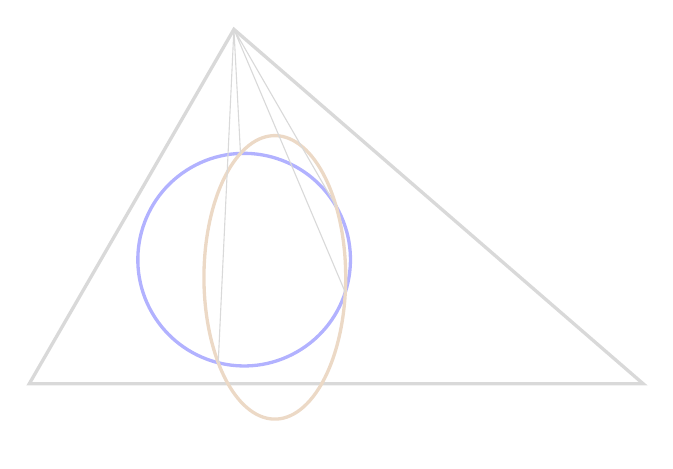
\begin{tikzpicture}[scale=3]
\newcommand{\lineclr}{gray!30}
\draw[\lineclr,very thick] 
({cos(90)},{sin(90)}) -- 
({cos(90+120)},{sin(90+120)}) -- 
({2*cos(90+2*120)},{sin(90+2*120)}) -- cycle;
%\draw[\lineclr](0,0) circle(.5);
%\draw[\lineclr](-.5,-.25) circle(.25);
\newcommand{\Bclr}{blue!30}
\newcommand{\Cclr}{brown!30}
\draw[\Bclr,very thick,name path=Bellipse] ({.5*cos(90)+.5*cos(90+2*120)},{.5*sin(90)+.5*sin(90+2*120)}) arc (30:390:.45);
\draw[\Cclr,very thick,name path=Cellipse] ({.5*cos(90)+.5*cos(90+2*120)},{.5*sin(90)+.5*sin(90+2*120)}) arc (30:390:.3 and .6);
%\draw [name path=ellipse] (2,0.5) ellipse (0.75cm and 1cm);
%\draw [name path=rectangle, rotate=10] (0.5,0.5) rectangle +(2,1);
\draw [\lineclr, name intersections={of=Bellipse and Cellipse}]
(intersection-1) -- ({cos(90)},{sin(90)}) 
(intersection-2) -- ({cos(90)},{sin(90)}) 
(intersection-3) -- ({cos(90)},{sin(90)}) 
(intersection-4) -- ({cos(90)},{sin(90)}); 
%(intersection-2) circle (2pt) node {2}
%(intersection-3) circle (2pt) node {3}
%(intersection-4) circle (2pt) node {4};
\end{tikzpicture}
\end{document}
